\section{Results and Analysis}

\subsection{The Paper Airplane}

To perform the experiments, we constructed three ``The Arrow" paper airplanes each using half a sheet of GP Spectrum A4 Multi-Use paper, 
which is 0.103mm thick and 4.6 gram in weight. See Figure~\ref{fig:arrow} for a picture of The Arrow. The Arrow was chosen because
of its simple construction and rigid structure. We spent around two minutes to fold it from scratch, and obtained great consistency across 
all three models. Due to The Arrow's relatively large wing aspect ratio, it experiences minimal flapping motion during flight. As a result, the actual 
flight condition better resembles what is assumed in the theory. We also applied double-sided tape in the middle section to improve its rigidity.

\begin{figure}[hl]
  \centering
    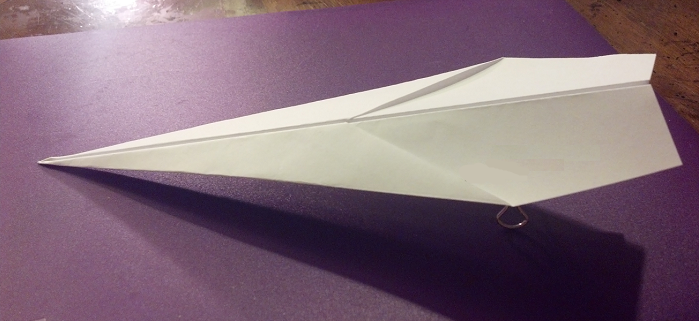
\includegraphics[scale=0.7]{figures/arrow.png}
    \caption{A picture of The Arrow. It is one of the most common paper airplane models. It has a long flight range and 
		         is easy to construct.}
  \label{fig:arrow}
\end{figure}

The Arrow measures $10000$mm in length and $100000$mm in width, and has a narrow delta wing shape. See Figure~\ref{fig:arrowdimension} for the detailed
dimension measurements. Each of the tests was performed with all three paper airplanes in order to reduce model specific errors. All launches were conducted
manually and an iPhone application was developed to record the launching speed.
 
\begin{figure}[hl]
  \centering
    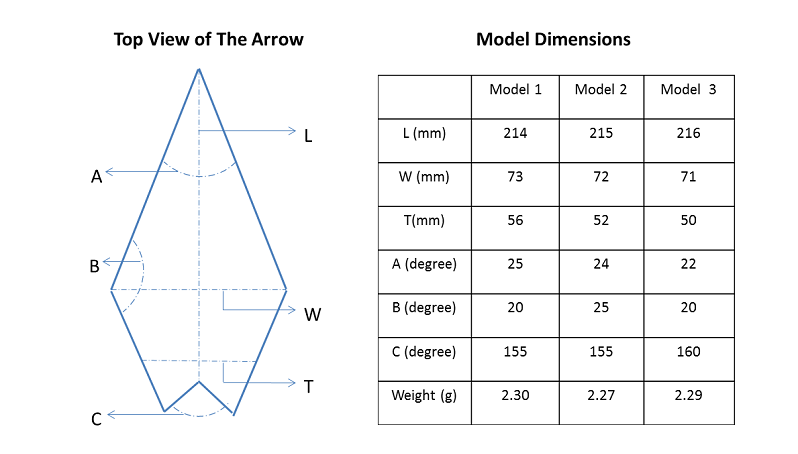
\includegraphics[scale=0.7]{figures/arrowdimension.png}
    \caption{Dimension of The Arrow used in the experiments. The measurements apply to all three models constructed.}
  \label{fig:arrowdimension}
\end{figure}


\subsection{Stability vs Center of Gravity}
We attached a metal clip $100$g in weight to various positions in the middle section of The Arrow to shift its center 
of gravity (see Figure~\ref{fig:}). We then launched The Arrow at specific height and speed. To measure its stability, we counted the 
number of complete yaws, rolls, and pitches the airplane completed in the air.  


\subsection{Stability vs Wing Angles}
aa
\subsection{Laminar-Turbulent Flow Transition}
aa
\subsection{Drag vs Lift Coefficient}
aa
\subsection{A Comparison of Different Paper Airplane Models}
aa